% Dette er utf8 udgaven af latex-templaten. Den er til brug på
% systemer der kører utf8x, såsom linux. Hvis du bruger windows, så er
% det letteste at hente windowsudgaven i stedet, da den i forvejen er
% gemt i latin1 format og har dette sat i inputenc. Hvis du ikke
% benytter danske tegn (æ,ø,å), så er det lige meget.
% 
% Loader dokumentklassen memoir. Sætter sproget i dokumentet til
% dansk, papirtypen til A4, sætter dokument til lige store højre og
% venstre margen, laver to søjler og siger at vi gerne vil lave en
% artikel, sætter skriftstørrelse til 9pt.
\documentclass[danish,a4paper,twoside,11pt]{memoir}
\setsecnumdepth{subsection}
\settocdepth{subsection}

\usepackage[danish]{babel} %Giver mulighed for dansk orddeling. Slet
% kun hvis du VED hvad du laver, eller skal
% skrive noget på engelsk.
\usepackage[utf8x]{inputenx} %Hvis du benytter windows i stedet for
% linux, så skift utf8 ud med
% latin1. Tillader danske tegn.
\usepackage{graphicx} %Tillader indsættelse af billeder
\usepackage{caption}
\usepackage{mathtools} %Ekstra matematik... bare lad den være, du får
% muligvis brug for den.
\usepackage{siunitx} %Bruges til at indsætte SI enheder med
% makroer. Sørger for at de kommer til at stå med
% rigtig skrifttype (normal skrift i
% matematik). Brug den, eller lad være. ²
% indsættes med \squaren for at undgå sammenfald
% med \square fra ams.
% \usepackage{url} %bruges til at formattere url'er... kan sagtens udelades.
\usepackage[version=3]{mhchem}
%\usepackage[hidelinks=true]{hyperref}
\usepackage{microtype} % Pakke der proever at fikse badbox
% problemer. Kun kompatibel med pdflatex.
%\renewcommand\ttdefault{txtt}
\usepackage[scaled]{luximono}

\usepackage{suffix}
\usepackage{wasysym}
\usepackage{multirow}
\usepackage{xspace}
\usepackage[caption=false]{subfig}
\let\subbottom\subfloat

\usepackage[flushleft]{threeparttable}
\usepackage[draft]{fixme}
\renewcommand\fxdanishfatalname{Fatal}

\usepackage[square,sort,comma,numbers]{natbib}

\usepackage{git-info}
\usepackage{stringstrings}



%%%% Forside stuff
\usepackage{mathpazo}% palatino + matematik
\usepackage{bm}
\usepackage{soul} % lege lege

%\usepackage{autonum}
\usepackage[hidelinks]{hyperref}
\usepackage{breakurl}
\usepackage{cleveref}



%%%%%%%%%%%%%%%%%%%%%%%%%%%%%%%%%%%%%%%%%%%%%%%%%%%%%%%%%%%%%%%%%%% 
%%%%%%%%%%%%%%%%%%%%%%          Forside          %%%%%%%%%%%%%%%%%%
%%%%%%%%%%%%%%%%%%%%%%%%%%%%%%%%%%%%%%%%%%%%%%%%%%%%%%%%%%%%%%%%%%%

\sodef\an{}{0.2em}{.9em plus.6em}{1em plus.1em minus.1em}
\newcommand\stext[1]{\an{\scshape#1}}
\pagestyle{simple} %Giver tom footer og sidetal i header
\usepackage{calc}
\newif\ifNoChapNumber
\makeatletter
\makechapterstyle{VZ34}{
  \setlength{\beforechapskip}{0.1pt}
  \setlength{\midchapskip}{1.0\onelineskip}
  \setlength{\afterchapskip}{1.5\onelineskip}
  \renewcommand\chapternamenum{}
  \renewcommand\printchaptername{}
  \renewcommand\printchapternum{}
  \renewcommand\chapnumfont{\Huge\bfseries}
  \renewcommand\chaptitlefont{\Huge\bfseries\raggedright}
  \renewcommand\printchaptertitle[1]{%
    \begin{tabular}{@{}p{1cm}|!{\quad}p{\textwidth-1cm-2em-4\tabcolsep }}
      \ifNoChapNumber\relax\else\chapnumfont \thechapter\fi
      & \chaptitlefont ##1
    \end{tabular}
    \NoChapNumberfalse
  }
  \renewcommand\printchapternonum{\NoChapNumbertrue}
}
\chapterstyle{VZ34}
%\chapterstyle{tandh}

%%%%%%%%%%%%%%%%%%%%%%%%%%%%%%%%%%%%%%%%%%%%%%%%%%%%%%%%%%%%%%%%%%%
%%%%%%%%%%%%%%%%%%%%%% Costumized math functions %%%%%%%%%%%%%%%%%%
%%%%%%%%%%%%%%%%%%%%%%%%%%%%%%%%%%%%%%%%%%%%%%%%%%%%%%%%%%%%%%%%%%%

\renewcommand{\d}[2]{\frac{d #1}{d #2}} % for derivatives
\newcommand{\dd}[2]{\frac{d^2 #1}{d #2^2}} % for double derivatives
\newcommand{\pd}[2]{\frac{\partial #1}{\partial #2}} 
% for partial derivatives
\newcommand{\pdd}[2]{\frac{\partial^2 #1}{\partial #2^2}} 
% for double partial derivatives
\newcommand{\pddd}[2]{\frac{\partial^3 #1}{\partial #2^3}}
\newcommand{\mvec}[1]{\bm{#1}}

\graphicspath{{./Figures/}{./Figures/Dalitz/}{./Figures/AlphaSpec/}}
\setkeys{Gin}{width=0.9\columnwidth}



%%% Grundstoffer
\newcommand{\Pu}{\ce{^{239}Pu}\xspace}

%Be-8
\newcommand\Be{\ce{^{8}Be}\xspace}
\WithSuffix\newcommand\Be*{\ensuremath{\ce{^{8}Be^*}}\xspace}

% Be-8
\newcommand\Bor{\ce{^{11}B}\xspace}
\WithSuffix\newcommand\Bor*{\ensuremath{\ce{^{11}B^*}}\xspace}

% C-12
\newcommand\Carb{\ce{^{12}C}\xspace}
\WithSuffix\newcommand\Carb*{\ensuremath{\ce{^{12}C^*}}\xspace}

%%% Siunitx
\sisetup{separate-uncertainty=true,
  quotient-mode = fraction,
  free-standing-units = true,
  use-xspace = true,
  space-before-unit = true}

\DeclareSIUnit\um{\micro\meter}
\DeclareSIUnit\MV{\mega\V}
\DeclareSIUnit\ub{\micro\barn}
\DeclareSIUnit\mb{\milli\barn}


%%%% Små ord
\newcommand{\beamline}{strålerøret\xspace}
\newcommand{\target}{folie\xspace}
\newcommand{\lAND}{\texttt{OG}\xspace}
\newcommand{\lOR}{\texttt{ELLER}\xspace}

\hyphenation{%
pro-ton-ener-gi-er %
Ruther-ford-spred-ning %
dob-belt-ko-in-ci-dens-spek-tre-ne %
trip-pel-ko-in-ci-dens-spek-tre-ne %
mod-strid-en-de %
}

%%%% Git stuff
\gitNewDateFormat{timeonly}{#4:#5}
\newcommand{\gitid}{\substring{\gitinfo{@head}{commit}}{1}{7}\xspace}
\newcommand{\gittime}{\gitinfo{@head}{dt@today}{} \gitinfo{@head}{dt@timeonly}\xspace}


%%%%%%%%%%%%%%%%%%%%%%%%%%%%%%%%%%%%%%%%%%%%%%%%%%%%%%%%%%%%%%%%
%%%%%%%%%%%%%%%%%% Header setup %%%%%%%%%%%%%%%%%%%%%%%%%%%%%%%% 
%%%%%%%%%%%%%%%%%%%%%%%%%%%%%%%%%%%%%%%%%%%%%%%%%%%%%%%%%%%%%%%% 


% \includeonly{%
% %  Bachelor-abstract,
% %  Bachelor-indledning,
% %  Bachelor-opstilling,
% %  Bachelor-eksparb,
%   Bachelor-kalibrering,
% %  Bachelor-rutherford,
% %  Bachelor-henfald,
% %  Bachelor-konklusion
% }
\begin{document}


\begin{titlingpage}
  \thispagestyle{empty}
  \centering
  { \setlength{\baselineskip}{24pt}
    {\Huge \stext{Carbon-12's} \par
      %\textit{for}\par
      \stext{henfaldsprocess}
    }\par
    \stext{(The decay process of carbon-12)}
    \par\vspace*{4\onelineskip}
    \par
    \includegraphics[width=8cm]{forside} 
    \par\vspace*{5\onelineskip}
    \stext{Bachelorprojekt i Fysik}\par
    \large\stext{Michael Kulmback Munch \par 20103561}\par
  }
  \vfill
  \vspace*{2\onelineskip}
  \stext{Vejleder: Hans Fynbo}\hfill
  \stext{1. juli 2013}
  \par\vspace*{2\onelineskip}
  \small
  \stext{Institut for Fysik og Astronomi}\par
  \stext{Aarhus Universitet}
  \enlargethispage{2\onelineskip}

  \newpage
  \thispagestyle{empty} % fjerne evt. sidehoved og -fod
  \small
  % resten af teksten indenfor dette env skal være \small
  \strut\vfill  % pres alt ned i bunden af siden
  \begin{flushleft}
    Institut for Fysik og Astronomi \par
    Aarhus Universitet \par
    Ny Munkegade, Bygning 1520 \par
    DK-8000 Aarhus C \par
    Danmark \par
    \vspace{\onelineskip}
    
    \copyright\ Michael Munch 2013                      \par
    \fxfatal{Not done yet}
    Forsidebilledet er et Dalitzplot.
  \end{flushleft}
\end{titlingpage}
%\cleardoublepage
\thispagestyle{empty} % ingen sidehoved eller -fod
\vspace*{\stretch{3}} % speciel faktoriseret gummilængde
\begin{center}
Tak til Hans og Kasper for deres tålmodighed.
\end{center}
\vspace*{\stretch{17}}
% ting efter siden skal starte på en højre side
\cleardoublepage
     
\frontmatter

\begingroup
\let\clearpage\relax
\vspace*{-5.5\onelineskip}
\chapter{Abstract}
\label{cha:abstract}
\vspace{-0.5\onelineskip}

In the course of the 20th century the $p + \Bor \rightarrow \Carb*$ reaction have been studied in
considerable detail because this reaction allows to study several questions, such as the decay
mechanism to the $3\alpha$ final states, and position of resonances in \Carb. This reaction is also a
candidate for fusion energy reactors, with the advantage that no neutrons are produced.

In this project this reaction has been studied with four segmented solid state detectors. This allows
for simultaneous detection of the energy and position of the daugther particles. This type of
detector is rather new, so an important part and motivation for the project was to understand the
detectors. Methods to overcome difficulties with these detectors is presented.

It was found that \Carb decays to three $\alpha$-particles via states in \Be. It has been determined that
the state at \SI{17.8}{\MeV} in \Carb is either a $0^{+}$ or $2^{+}$ state. From the spectrum it was
possible to deduce that decay via the excited state in \Be is more probable than decay via the
groundstate. These observations are consistent with the literature \cite{States}.

Furthermore the results suggest that at \num{18.2} and \SI{18.5}{\MeV} \Carb is in a $0^{+}$ or
$2^{+}$ state which contradict the literature. The conclusion is that there is no $1^{+}$ state at
\SI{18.2}{\MeV}, but the results were not conclusive for the \SI{18.5}{\MeV} state.

These results shows that segmented solid state detectors provides an improved tool for observing
nuclear processes with multiple decay fragments. 

\vspace{1\onelineskip}
\chapter{Resume}
\label{cha:resume}
\vspace{-0.5\onelineskip}

I løbet af det 20. århundrede er $p + \Bor \rightarrow \Carb*$ reaktionen blevet studeret i stor
detalje, da den giver mulighed for undersøge adskillige spørgsmål, såsom henfaldsmekanismen til $3\alpha$
sluttilstande og positionen af resonanser i \Carb. Desuden er reaktionen også en kandidat til
fremtidens fusionsreaktorer, da den ikke producerer frie neutroner. 

I denne rapport er reaktionen undersøgt ved at anvende fire segmenterede faststofdetektorer, som
muliggør energi- og positionsfølsom dektektion. Denne type detektorer er forholdsvis ny, så en
vigtig del og motivation for projekt var at forstå disse detektorer. Der vil blive redegjort for
løsningen problemer i forbindelse med detektorsystemet.

% Der vil blive redegjort for disse, samt metoder til at løse disse
% vaskeligheder. \fxfatal{Indforstået - flere ord}

Resultatet af undersøgelserne er, at \Carb henfalder til tre $\alpha$-partikler via en tilstand i
\Be. Det kan konkluderes, at der findes en $0^{+}$ eller $2^{+}$ tilstand ved \SI{17.8}{\MeV} i
\Carb. Endvidere blev det observeret, at tværsnittet for henfald til grundtilstanden er større end for
henfald til den exciterede tilstand. Dette stemmer overens med litteraturen \cite{States}.

Undersøgelserne indikerer også en $0^{+}$ eller $2^{+}$ tilstand ved hhv. \num{18.2} og
\SI{18.5}{\MeV}, hvilket er i strid med litteraturen. For tilstanden ved \SI{18.2}{\MeV} er
fortolkningen, at den rapporterede $1^{+}$ tilstand ikke findes. Resultaterne for \SI{18.5}{\MeV} er
dog ikke endegyldige.

Resultaterne viser, at segmenterede faststofdetektorer giver mulighed for at observere
nukleareprocesser med flere datterkerner med større præcision end hidtil muligt. 




\endgroup

\cleardoublepage
\begingroup
\setlength\cftparskip{-2pt}
\tableofcontents
\vspace{2cm}
\endgroup

\begingroup
\let\clearpage\relax
\vspace*{5mm}
\chapter{Forord}
Denne rapport er udarbejdet af Michael Kulmback Munch som afsluttende bachelorprojekt
i Fysik ved Aarhus Universitet. Dataopsamlingen er foretaget sammen med Kasper Lind Jensen under
vejledning af lektor Hans Fynbo. Opstillingen er en del af LOBENA-projektet.

Fokus i denne opgave er på forståelse af detektorsystemet og kalibrering af dette, samt at opnå
viden om placering af resonanser i \Carb.

Jeg vil gerne sige tak til Anne-Sofie Greve, Emil Eriksen og Lars Munch for gennemlæsning og
rettelser til opgaven og Hans Fynbos tålmodighed under vejledningsprocessen. 

\vspace{2\onelineskip}
\noindent
\rule{7cm}{0.4pt}


\endgroup
%\listoffixmes

\mainmatter
\chapter{Indledning}
\label{cha:indledning}

\chapter{Opstilling}
\label{cha:opstilling}

Et beam af protoner accelereres op til den ønskede energi med en 5\MeV Van de Graaf
accelerator. Dette beam afbøjes med en eletromagnet og sendes ind i beamline, hvor det først
passerer gennem et hul i midten af den ene detektor, hvorefter en del af det vil kolliderer med et
\ce{^{11}B}-target på carbon backing.
\fxfatal{Hvad er tykkelsen af foliet og backing?}
Det resterende vil passere videre gennem beamline, hvor det
igen vil passere gennem en detektor, for at ende i en Faraday cup.

Detektorsystemet består af to dobbel siddet silicium strip detektorer (DSSSD), som fungerer på samme
måde, som almindelige fasstofdetektorer. Fordelen er opdelingen af forsiden og bagsiden i et antal
områder kaldet strips. Dermed er det muligt at bestemme både vinkel og energi af
partiklerne. Bagsiden er opdelt i 32 radiale slices, som benævnes sektorer. Forsiden er derimod
opdelt i en række ringe, der hver er 886\um tykke, med et 100\um isolerende område mellem hver.

Den første detektor beamet passerer igennem kaldes upstream. Denne udspænder vinklerne fra
$141\degree$ til $165\degree$ målt fra beamets retning. Den anden benævnes med downstream og den
udspænder fra $15\degree$ til $40\degree$.


\begin{figure}[h]
  \centering
  \fxfatal{Skematisk tegning af opstillingen mangler.}
  %\includegraphics{}
  \caption{Skematisk tegning af opstillingen}
  \label{fig:opstilling}
\end{figure}

\chapter{Det eksperimentelle arbejde}
\label{cha:eksp}

Det eksperimentelle arbejde begyndte i januar 2013. På dette tidspunkt var kun de to S3 detektorer
monteret. Her blev foretaget målinger med protonenergier mellem \num{0.5} og \SI{2.4}{\MeV}, hvor
det logiske kredsløb var indstillet til både \lAND og \lOR. Dette gav mulighed for at undersøge både
Rutherfordspredning og $\alpha$-henfald. Detektionsraten, når det logiske kredsløb var indstillet på \lOR,
var mellem 10 og 20\kHz. Af disse blev cirka 20\% afvist, da de ankom, mens analog-til-digital
konverteringen var i gang. Med det logiske kredsløb indstillet til \lAND blev ingen hændelser afvist,
da detektionsraten kun var omkring 200\Hz. Sandsynligheden for, at $\alpha$-partikler blev afvist, fordi
ADK'en var optaget, var derfor meget mindre.

Til at foretage en kalibrering mellem energi og kanalnumre blev der benyttet tre $\alpha$-kilder. Det
viste sig dog hurtigt, at der var problemer med kalibreringen. Hvis der blev benyttet 2\MeV
protoner, forekom den tilsvarende Rutherfordtop i spektret for den inderste ring i detektor 4 ved
\SI{2.6}{\MeV}. Forklaringen på dette var, at detektorerne havde et inaktivt område, et såkaldt
dødlag, hvor partiklerne tabte energi, før de blev detekteret. Fordi kalibreringskilden var en
$\alpha$-kilde og stoppeevnen af disse er større end protoners, blev der overkompenseret for dødlaget.

På baggrund af denne observation blev der foretaget nye målinger med kalibreringskilden, så
tykkelsen af det inaktive område kunne fastslås. Selve proceduren findes i
\cref{cha:kalibrering}. Resultatet af målingerne viste, at dødlaget på den side af detektorerne, der
hidtil havde vendt ind mod foliet, var væsentligt tykkere end det på bagsiden af detektorerne. 

For at mindske usikkerheden blev detektorerne roteret og kalibreret, hvor der blev taget hensyn til
dødlaget.  I mellemtiden var de to W1 detektorer også blevet tilføjet. Kalibreringerne af alle
detektorerne bliver verificeret i \cref{cha:rutherford}. De originale data blev kasseret og nye
målinger ved 2, \num{2.37} og \SI{2.65}{\MeV} blev foretaget. Disse nye data blev alle
indsamlet med det logiske kredsløb indstillet til \lAND og over et længere tidsrum for at øge
datamængden. Den eneste ulempe var, at der ikke blev foretaget målinger over et ligeså bredt
energiinterval. Analysen af disse data findes i \cref{cha:sekventielt-henfald}.

\section{Analysearbejdet}
\label{sec:analyse}

Til analysearbejdet blev analyseværktøjet ROOT benyttet. ROOT er udviklet på CERN og er en række
udvidelser til programmeringssproget C++. De rå datafiler blev konverteret til en ROOT specifik
datastruktur, kaldet et ROOT-træ. Indlæsning af data foregår med en standardalgoritme og foregår en
hændelse ad gangen. For hver hændelse registreres for hver detektor antal detektioner i
forsiden og bagsiden af detektoren, de ramte strips samt kanalnummeret for de enkelte
detektioner. Opgaven var  at rekonstruere de fysiske begivenheder ud fra disse tal.

Først og fremmest er det nødvendigt at foretage en kalibrering for hver enkelt strip, så
kanalnumrene kan oversættes til kinetisk energi. Endvidere kan både azimut- og polarvinklen
rekonstrueres ud fra den ramte for- og bagstrip. Dette gøres ud fra både detektortypen og afstanden
til detektoren. Det er ikke muligt at bestemme afstanden til detektorerne med stor nøjagtighed, da
opstillingen er meget kompakt og detektorerne skrøbelige. Derfor var det nødvendigt at justere
parametererne for placeringen af de forskellige detektorer indtil resultaterne var selvkonsistente
samt konsistent med veletableret fysik, såsom energiens vinkelafhængighed for Rutherfordspredte
protoner. Dette er beskrevet i \cref{cha:rutherford}.

For hver hændelse blev energien og vinklerne af de enkelte partikler beregnet. Resultaterne i dette
projekt er fundet ved kombinere disse informationer som beskrevet i hhv. \cref{sec:ruther-data} og
\ref{sec:sek-data}.

Koden brugt til analysen er skrevet fra bunden i løbet af projektet.

\chapter{Kalibrering}
\label{cha:kalibrering}

For at kunne oversætte mellem udstyrets kanalnummer og en given energi skulle der foretages en
kalibrering. Til dette formål blev der benyttet en kilde, der bestod af tre $\alpha$-kilder:
\ce{^{241}Am}, \ce{^{239}Pu} og \ce{^{244}Cm}.

Da forstærkningen er indstillet forskelligt i de enkelte strips og sektorer, er det nødvendigt at
kalibrere dem enkeltvisn. Linierne er skarpt adskilte og kalibreringen kan udføres ved at fitte
lineært til de pågældende centroid værdier.

Det skulle dog vise sig at være mere vanskeligt end først antaget, da detektoren havde et inativt
område, der blot bremsede partiklen uden at registrere energien. Dødlaget havde en tykkelse
$\Delta x$ på et par mikrometer, hvilket er illustreret på \cref{fig:deadLayer}.

Dødlaget har den effekt, at partikler, der rammer længere ude på detektoren, vil miste mere energi
end dem, der rammer de inderste strips, da de skal igennem en større vejlængde i dødlaget.

De relevante størrelser er den målte energi $E_{0}$, energien før dødlaget $E$ og vinklen $\phi$ mellem
partiklens hastighed og detektorens normal. Ud fra nogle enkelte geometriske betragtninger kan et
udtryk for $E$ opskrives
\begin{equation}
  \label{eq:deadE}
  E = E_{0} + \d{E}{x} \frac{\Delta x}{\cos \phi}  .
\end{equation}
Det sidste led er energitabet i dødlaget, som afhænger af materialets stoppeevne $\d{E}{x}$. Denne
antages at være konstant gennem dødlaget.

Det skal bemærkes, at dette er en approksimation, da producenten har oplyst, at dødlaget består både
af aluminium og silicium. Disse grundstoffer er hhv. nummer 13 og 14 i det periodiske system, så er
deres stoppeevne er stort set ens, og dødlaget approksimeres derfor til et enkelt lag silicium.
\begin{figure}[h]
  \centering
  \includegraphics[width=7cm]{DeadLayer}
  \caption{Skematisk tegning af S3 dektoren med et dødlag.}
  \label{fig:deadLayer}
\end{figure}

\section{Estimering af dødlagets tykkelse}
\label{sec:dodlag}

For at kunne bestemme tykkelsen af dødlaget er det nødvendigt at kende energien ved forskellige
vinkler, men som tidligere nævnt er forstærkningen indstillet forskelligt i ringene.

Løsningen på dette er at udvælge en radial sektor. Hver gang denne sektor bliver ramt, findes den
tilsvarende cirkulære strip. Kriteriet for dette er, at kanalnumrerne stemmer overens inden for en
vis tolerance. Dermed er det muligt at bestemme spektret for de enkelte cirkulære strips udtrykt i
kanalnummeret for den radiale sektor og derfor er der ingen forstærkning at tage højde for i
spektrene.

I alle disse spektre bestemmes centroidværdien af \Pu toppen.  Centroidværdien normaliseres til
kanalnummeret i strip 1 og plottes som funktion af $1/{\cos \phi}$. Ud over dette er
\cref{eq:deadE} også plottet for forskellige tykkelser. Disse er normaliseret til det teoretiske
udtryk for strip 1. Stoppeevnen er taget fra \cite{Ziegler}.

Det er ikke muligt at lave et fit til data med $\Delta x$ som en fri parameter, så tykkelsen af
dødlaget er vurderet ud fra de teoretiske kurver, som er plottet på \cref{fig:dead}. Data er
konsistent med en tykkelse på hhv. \SI{3.3(5)}{\um} og \SI{4.2(5)}{\um} for detektor 4 og 3. En
tilsvarende analyse er foretaget med S3 detektorerne roteret 180\degree. Her er resultatet, at
dødlaget var væsentlig mindre blot \SI{0.6(1)}{\um}. 

\begin{figure}[h]
  \centering
  \subbottom[Detektor 3]{\includegraphics[width=0.47\columnwidth]{DeadLayerThin}}%
  \hfill
  \subbottom[Detektor 4]{\includegraphics[width=0.47\columnwidth]{DeadLayerThick}}%
  \caption{De normaliserede energier som funktion af $1/{\cos\phi}$. Kurverne angiver det teoretiske
    udtryk givet i \cref{eq:deadE} og er plottet for forskellige tykkelser.}
  \label{fig:dead}
\end{figure}

\vspace{-5mm}
\section{Kalibreringsalgoritmen}
\label{sec:kalalgo}

Når tykkelsen er kendt, kan den målte energi $E_{0}$ bestemmes. Dermed kan vores detektorer
kalibreres. Under databehandlingen er det nødvendigt at bestemme energitabet for hver enkelt
hændelse, da energitabet afhænger af både indgangsenergien og partikeltypen.

For energier, hvor stoppeevnen er stor, vil det give anledning til fejl, hvis energitabet anses som
konstant hele vejen igennem materialet. Det samlede tab skal derfor udregnes ved integration og
i stedet benyttes middelrækkevidden for en partikel i et givent materiale. Ækvivalent til
\cref{eq:deadE} kan den samlede rækkevidde skrives som
\begin{equation}
  \label{eq:deadR}
  R(E) = R(E_{0}) + \frac{\Delta x}{\cos \phi} .
\end{equation}

Rækkeviden som funktion af energien er også tabuleret i \cite{Ziegler}, så for en given hændelse
blev $R(E_{0})$ bestemt ved lineær interpolation mellem de to nærmeste tabulerede værdier. Til dette
adderes tykkelsen af dødlaget, hvor der blev taget højde for vinklen. Den samme tabel blev også
benyttet den modsatte vej, hvor energien blev bestemt ud fra den samlede rækkevidde. Der blev igen
benyttet lineær interpolation.

Denne algoritme er anvendt til at lave \cref{fig:kalib-spec}, der viser det kalibrerede spektrum i
hhv. den inderste og yderste ring i detektor 3. 

\section{Resultater}
\label{sec:kalib-resultater}

I dette kapitel er der fremlagt data, der indikerer, at S3 detektorerne har et dødlag. På baggrund
af denne observation er der fremlagt en metode til at estimere tykkelsen af dødlagene. Med denne
metode blev det etableret, at dødlaget på bagsiden af detektorerne var 6-7 gange mindre end
forsidens og data i resten af rapporten vil være med detektorerne roteret 180\degree. Desuden er
der også præsenteret en kalibreringsalgoritme, der korrigerer for dødlaget. At algoritmen virker
efter hensigten vil blive verificeret i næste afsnit.

\begin{figure}[hb]
  \centering
  \vspace{-0.2cm}
  \subbottom[Inderste ring.]{\includegraphics[width=0.4\columnwidth]{kalib-spec-inner}}%
  \hfill
  \subbottom[Yderste ring.]{\includegraphics[width=0.4\columnwidth]{kalib-spec-outer}}%
  \caption{Energispektrum for henfaldskilden for detektor 3 med forsiden vendt mod kilden. Her er
    antaget, at dødlaget er \SI{4.2}{\um}.}
  \label{fig:kalib-spec}
  \vspace{-4cm}
\end{figure}










\chapter{Kinematiske kurver}
\label{cha:rutherford}

I dette afsnit udledes og præsenteres de kinematiske kurver, dvs. energien som funktion af vinklen,
for hhv. Rutherfordspredning og $\alpha$-partiklen frigivet ved processen
$\Carb* \rightarrow \Be + \alpha$. Disse kurver kan ekstraheres fra data ved brug af
kalibreringsalgoritmen beskrevet i \cref{sec:kalalgo} og benyttes til at vise overensstemmelse
mellem kalibreringen og teorien.

\section{Teori}
\label{sec:teori}

\begin{figure}[b]
  \vspace{5mm}
  \centering
  \includegraphics[width=0.4\columnwidth]{Rutherford-kin}
  \caption{Principskitse af impulserne i spredningsprocessen $b + t \rightarrow b' + t'$ set fra massemidtpunktssystemet.}
  \label{fig:ruther-kin}
  \vspace{-5mm}
\end{figure}

\Cref{fig:ruther-kin} skitserer den generelle spredningsproces
\begin{equation}
  \label{eq:spredning}
  b + t \rightarrow b' + t'.
\end{equation}

Den kinetiske energi af den udkommende partikel $b'$ i laboratoriesystemet (LAB) er givet ved
\begin{equation}
  \label{eq:udkommendeE}
  T_{b'} = \frac{1}{2}m_{b'} \mvec{V_{b'}}^{2} = \frac{1}{2}m_{b'}(V_{CM}^{2} + V_{b'}'^{2} +
  2V_{CM}V_{b'}'\cos \theta' ),
\end{equation}
hvor $V'$ angiver hastigheder i massemidtpunktssystemet (CM) og $\theta'$ vinklen mellem $b'$ og $t$.

Begrænser man sig til at se på Rutherfordspredning svarende til at $t' = t$ og $b' = b$, så må
$V_{b'}' = V_{b}'\,$, da Coulombkraften er konservativ. Denne kan bestemmes ud fra energien af strålen
$T_{b}$
\begin{equation}
  \label{eq:rutherUdCM}
  V_{b}' = \frac{\mu}{m_{b}}V_{b} = \frac{m_{t}}{m_{t}+m_{b}} \sqrt{\frac{2T_{b}}{m_{b}}},
\end{equation}
hvor $\mu$ betegner den reducerede masse. Indsættes denne i \cref{eq:udkommendeE} kan energien
udtrykkes ved kun én fri variabel
\begin{equation}
  \label{eq:rutherUdLab}
  T_{b} = T_{b} \frac{m_{b}}{(m_{t}+m_{b})^{2}} \Bigl(m_{b} + \frac{m_{t}^{2}}{m_{b}} + 2m_{t}\cos \theta'\Bigr).
\end{equation}
Rutherfordspredning i LAB-systemet vil derfor give anledning til et kontinuert spektrum givet ved
\cref{eq:rutherUdLab}. I CM er energien bestemt af energi- og impulsbevarelse og givet ved
\cref{eq:rutherUdCM}.

I det generelle tilfælde er det ikke så ligetil. Her udnyttes, at i CM skal
$\mvec{p_{t'}} + \mvec{p_{b'}} = \mvec{0}$. Endvidere skal den samlede energi af $b'$ og $t'$ være
lig energien $E_{CM}$, som ikke er bundet i massemidtpunktets bevægelse. Kombinerer man dette med
\cref{eq:rutherUdCM}, får man
\begin{equation}
  V_{b'}'^{2} = \frac{2E_{CM}}{m_{b'}(1+\frac{m_{b'}}{m_{t'}})}.
\end{equation}
Indsættes dette i \cref{eq:udkommendeE} er det muligt at bestemme energien af $b'$ i LAB-systemet ud
fra $\theta'$
\begin{align}
  T_{b'} = m_{b'} \Bigl(T_{b}&\frac{m_{b}}{(m_{t} + m_{b})^{2}} + \frac{E_{CM}}{m_{b'}(1+\frac{m_{b'}}{m_{t'}})} \notag\\
  &+ 2 \sqrt{T_{B}E_{CM} \frac{m_{b}}{m_{b'}}}\bigl[(m_{t} + m_{b})(1 + \frac{m_{b'}}{m_{t'}})^{1/2}\bigr]^{-1} \cos \theta'\Bigr).
  \label{eq:alphaUdLab}
\end{align}
Som ved Rutherfordspredning giver denne proces også anledning til et kontinuum i LAB-systemet og
en veldefineret energi i CM. 


\section{Data og databehandling}
\label{sec:ruther-data}

Databehandlingen af dette forsøg er simpel. For hver detekteret partikel bestemmes polarvinklen ud
fra hvilken detektor og forstrip, der rammes. For de firkantede detektorer er det også nødvendigt at
bestemme bagstrippen. Her findes den bagstrip, hvor energiforskellen er mindst mulig. Detektionen
afvises, hvis forskellen er større end 100\keV. Energien og polarvinklen tilføjes til et
2D-histogram.

\subsection{Tyndt folie}
\label{sec:tyndtfolie}

For at undgå andre processer end Rutherfordspredning er her benyttet et \SI[per-mode =
symbol]{4}{\micro\gram\per\cm\squared} kulstoffolie. Resultatet ses på \cref{fig:1072}, hvor
rækkevidden for protoner er anvendt. Som forventet fra teorien afhænger energien af den spredte
proton af spredningsvinklen og udgør et kontinuum i LAB-systemet.
\begin{figure}[htb]
  \centering
  \subbottom[LAB systemet]{\includegraphics[width=0.49\columnwidth]{AngleEnergy1072-LABd}}%
  \hfill
  \subbottom[CM for protonen]{\includegraphics[width=0.49\columnwidth]{AngleEnergy1072-CMp}}%
  \caption{Antal tællinger som funktion af energi og vinkel for spredning af protoner på
    kulstof. Den røde linie er \cref{eq:rutherUdLab} med $m_{t} = m_{\!\!\Carb}$. Fra venstre mod
    højre ses data fra detektor 4, 1 og 3. Større tæthed angiver højere antal tællinger.}
  \label{fig:1072}
\end{figure}

\Cref{fig:1072}b viser det tilsvarende data, hvor der er transformeret til CM for protonen. Dette
viser, hvorledes energien af den udgående proton i CM med god tilnærmelse er en konstant. De
små usikkerheder for de runde detektorer skyldes primært usikkerheder på detektorernes
positioner.

Det lader også til, at energien fra de firkantede detektorer ligger en smule under kurven. Det kan
skyldes, at disse har et lille dødlag, der skal tages højde for. Dette er der dog ikke gjort i
denne opgave.

Data viser endvidere, at foliet ikke kun består af \Carb, men også af andre
grundstoffer. 

Her er både tale om et enkelt let grundstof, der ses under den røde linie samt tungere grundstoffer
over linien. Disse fordeler sig således, da de lette grundstoffer får en højere rekylenergi ved
sammenstød med protonen. Dette kan muligvis skyldes vand på foliet. 

\subsection{\Bor folie}
\label{sec:tykt-folie}

Her ses på data fra protonbeskydning af det \Bor-folie, som er benyttet gennem resten af
eksperimentet. Her forventes ud over Rutherfordspredning også reaktionen
$p + \Bor \rightarrow \Carb*$. Dette kulstof er ustabilt og vil henfalde igen. I
\cref{cha:sekventielt-henfald} vil der blive redegjort for henfaldsprocessen i detaljer, specifikt
udledes i \cref{sec:tilstand} et udtryk for energien i CM
\begin{equation}
  E_{CM} = \frac{11}{12} T_{p} + Q = \frac{11}{12} T_{p} + m_{p} + m_{\!\!\Bor} - m_{\alpha} - m_{\Be},
\end{equation}
hvor det første led følger af $V_{CM} = \mu V_{b} / m_{b}$. 

\Cref{fig:1077} viser data og den teoretiske kurve givet ved \cref{eq:alphaUdLab}. Her er anvendt
rækkevidden for $\alpha$-partikler, hvilket er årsagen til, at Rutherfordlinien passer så
dårligt. Rutherfordlinien i de runde detektorer krummer opad mod områderne svarende til store
detektorvinkler. Dette skyldes overkompensation for dødlaget.  Den samme effekt ses også i $\alpha$-linien
i CM, hvilket tyder på, at dødlaget er tyndere end de estimerede \SI{0,6}{\um}.

På trods af disse små effekter stemmer spektret fint overens med de kinematiske kurver, hvilket
indikerer, at \Carb* kan foretage $\alpha$-henfald.

Det noteres, at \Bor foliet indeholder flere urenheder end bagbeklædningen.
\begin{figure}[ht]
  \centering
  \subbottom[LAB systemet]{\includegraphics[width=0.49\columnwidth]{AngleEnergy1077-LABd}}%
  \hfill
  \subbottom[CM for $\alpha$-partiklen]{\includegraphics[width=0.49\columnwidth]{AngleEnergy1077-CMa}}%
  \caption{Antal tællinger som funktion af energi og vinkel for spredning af protoner på \Be. Den
    øverste røde linie er \cref{eq:alphaUdLab} og den nederste er \cref{eq:rutherUdLab}. I begge
    tilfælde er $m_{t} = m_{\!\!\Bor}$. Fra venstre mod højre ses data fra detektor 4, 1 og
    3. Større densitet angiver højere antal tællinger.}
  \label{fig:1077}
\end{figure}

\section{Resultater}
\label{sec:ruther-konklusion}
Det er vist, at de eksperimentielt opnåede kinematiske kurver stemmer godt overens med de
teoretiske. Der er observeret afvigelser, der indikerer, at tykkelsen af dødlaget for S3
detektorerne er overvurderet en smule og W1 detektorerne muligvis har et lille dødlag. Størrelsen af
disse afvigelser er dog små. Kalibreringen kan derfor benyttes til den videre analyse.








\chapter{Henfaldprocessen af \Carb}
\label{cha:sekventielt-henfald}

I dette afsnit præsenteres den generelle teori for hhv. to- og tre-partikelhenfald. På baggrund af
teorien argumenteres for den sekventielle henfaldsmodel, som en måde at inkludere
$\alpha$-$\alpha$ vekselvirkninger i henfaldet. Dernæst præsenteres Dalitzplottet som et værktøj til at
identificere  resonanser og der redegøres for generelle egenskaber ved
Dalitzplottet. Til sidst præsenteres de eksperimentelle data. 

\section{Teoretisk baggrund}
\label{sec:sekventiel-teo}

For et henfald, hvor moderkernen deles i to, et såkaldt to-partikelhenfald {$M \rightarrow a + b$},
er der otte frihedsgrader - to impulsvektorer, hver med tre komponenter, samt to energier. Disse
størrelser er underlagt bevarelseslovene for energi og impuls, hvilket reducerer antallet af
frihedsgrader til nul. I et energispektrum vil et sådant henfald give anledning til to
toppe. Energierne af disse i massemidtpunktssystemet for moderkernen er givet ved
\begin{equation}
  \label{eq:toE}
  T_{a} = \frac{m_{b}}{m_{a} + m_{b}}Q, \qquad T_{b} = \frac{m_{a}}{m_{a} + m_{b}}Q.
\end{equation}

Tre-partikelhenfaldet, {$M \rightarrow a + b + c$}, har derimod 12 frihedsgrader - ni fra impuls og
tre fra energi. Dette kan reduceres ved at overveje følgende; henfaldet foregår i ét plan, så
$p_{i,z}$ kan sættes lig nul. Dette fjerner tre frihedsgrader. Energi- og impulsbevarelse eliminerer
tilsammen tre frihedsgrader. Energi-impuls relationen, $E^{2} = p^{2} + m^{2}$, anvendt for hver
enkelt datterkerne begrænser også tre frihedsgrader. En rotation i xy-planet ændrer ikke systemet,
hvilket fjerner én enkelt frihedsgrad. Antallet af frihedsgrader kan dermed reduceres til to,
hvilket betyder, at systemets tilstand afgøres af dynamikken, dvs. vekselvirkninger i systemet.

Henfalder \Carb-kernen direkte til tre ikke-vekselvirkende $\alpha$-partikler, vil energispektret
pga. de to frihedsgrader udgøre et kontinuum af energier. Denne proces kaldes direkte henfald og
er skitseret på \cref{fig:becker}a.

\begin{figure}
  \centering
  \includegraphics{Becker}
  \caption{Energidiagram for henfaldsprocessen af \Carb skitseret for hhv. (a) direkte henfald  og
    (b) sekventielt henfald. Figuren er lånt fra \cite{becker}.}
  \label{fig:becker}
  \vspace{-5mm}
\end{figure}

\subsection{Sekventielt henfald}
\label{sec:sekventielt-henfald}

En anden mulighed for tre-partikelhenfald er to på hinanden følgende to-partikelhenfald. Dette
benævnes sekventielt henfald. I tilfældet med \Carb henfalder den først til en tilstand i \Be under
udsendelse af en $\alpha$-partikel. Modsat det direkte henfald, som negligerer vekselvirkninger mellem
henfaldsprodukterne, svarer det sekventielle henfald til kraftig vekselvirkning mellem to af de tre
$\alpha$-kerner. Berylliumkernen vil derefter henfalde til to sekundære $\alpha$-partikler.

Det effiktive antal frihedsgrader er det samme som for det direkte henfald på trods af, at
sekventielt henfald blot er to to-partikelhenfald. Dette skyldes, at massemidtpunktssystemet for de
to henfald er forskellige. Set fra CM for det ene henfald vil det sekventielle henfald give
anledning til en top og et kontinuum.

% Med sekventielt henfald menes henfald fra den populerede tilstand i \Carb først med et primært
% henfald \Be samt en $\alpha$-partikel, hvor beryllium kernen foretager et sekundært henfald til to
% $\alpha$-partikler. Dette vil give andledning til et anderledes spektrum end et direkte henfald fra \Carb
% til tre $\alpha$-partikler, som giver andledning til et kontinuum af tilstande, der afgøres af vinklen
% mellem de enkelte $\alpha$-partikler, se \cite{Becker}.

Den sekventielle henfaldsproces er illustreret på \cref{fig:becker}b og tages der udgangspunkt i CM
for moderkernen, vil det sekventielle henfald af \Carb give anledning til en smal top ved energien
svarende til henfald via grundtilstanden af \Be
\begin{equation}
  \label{eq:alpha0}
  \Carb* \rightarrow \Be + \alpha_{0} \rightarrow 2\alpha_{2} + \alpha_{0}.
\end{equation}
Selvom \Be er ustabil, er grundtilstanden stadig ret smal med en bredde på kun
\SI{6.8}{\eV} \cite{States} og derfor vil bredden af toppen primært skyldes detektorens
opløsningsevne, som er 20\keV FWHM. 

Ved de anvendte protonenergier er der endvidere mulighed for at henfalde til den første exciterede
tilstand i \Be, der ligger \SI{2.95}{\MeV} over grundtilstanden
\begin{equation}
  \label{eq:alpha0}
  \Carb* \rightarrow \Be* + \alpha_{1} \rightarrow 2\alpha_{2} + \alpha_{1}.
\end{equation}
Bredden af denne top afgøres primært af bredden af \Be tilstanden, som er \SI{1.5}{\MeV}. Toppen vil
derfor approksimativt svare til en Breit-Wigner fordeling \cite[s. 26]{Martin}, som er væsenligt
breddere end den tilsvarende for $\alpha_{0}$ samt ligger ved lavere energi.

Der ligger endnu en tilstand \SI{11.35}{\MeV} over grundtilstanden. Sandsynligheden for at populere
denne er dog forsvindende lille ved de protonenergier, der benyttes. 

Idet begge berylliumtilstande er ustabile vil der pga. den korte levetid, forekomme endnu et
henfald udmiddelbart efter. Dette vil give anledning til to sekundære $\alpha$-partikler, hhv.
$\alpha_{21}$ og $\alpha_{22}$. Energien af disse kan bestemmes ud fra følgende kinematiske overvejelser.

\subsubsection{Kinematik}
\label{sec:sekv-kinematik}

En skitse af situationen efter det sekundære henfald ses på \cref{fig:secundary}.
\begin{figure}[h]
  \centering
  \includegraphics[width=0.6\columnwidth]{Sekventiel-kinematik}
  \caption{Skitse af situationen af det sekundære henfald. Vektorerne angiver hastighederne. $\phi$ er
    vinklen mellem hastigheden af beryllium og de sekundære $\alpha$-partikler i CM for beryllium. $\phi_{2i}$ er
    de tilsvarende vinkler i LAB-systemet.}
  \label{fig:secundary}
\end{figure}

Både i laboratorie- (LAB) og massemidtpunktsystemet (CM) følger af energi og impulsbevarelse,
at energien af de to primære henfaldsprodukter må være
\begin{equation}
  \label{eq:Ealpha0}
  E_{\alpha_{0}} = \frac{2}{3} Q_{1} \qquad E_{\ce{Be}} = \frac{1}{3} Q_{1},
\end{equation}
hvor $Q_{1}$ er den frigivne energi ved det primære henfald $\Carb \rightarrow \alpha + \Be$. Grundet
impulsbevarelse skal de to sekundære $\alpha$'er have lige stor og modsatrettet impuls i CM for
beryllium, Deres hastighed vil danne en vinkel $\phi$ i forhold til beryllium kernens
hastighed. Energien af de to er givet ved
\begin{equation}
  \label{eq:Ealpha2}
  E_{\alpha_{2}}' = \frac{1}{2} Q_{2},
\end{equation}
hvor $Q_{2}$ er den frigivne energi for det sekundære henfald. Hermed ses tydeligt, at i CM er
energien af de sekundære partikler konstant uanset vinklen.

De tilsvarende størrelser i LAB systemet kan bestemmes ved at tage højde for tyngdepunktets
bevægelse, som svarer til berylliumkernens bevægelse
\begin{align}
  E_{\alpha_{2}} %&= \frac{1}{2}m_{\alpha} (\mvec{V_{\ce{Be}}} + \mvec{V_{\alpha}})^{2} \notag \\
  &= \frac{1}{2}m_{\alpha} (V_{\ce{Be}}^{2} + V_{\alpha}^{2} + 2V_{\ce{Be}}V_{\alpha} \cos \phi) \notag \\
  &= \frac{Q_{1}}{6} + \frac{Q_{2}}{2} + \sqrt{\frac{Q_{1}Q_{2}}{3}} \cos \phi,           
  \label{eq:E2LAB} 
\end{align}
hvor der er anvendt approksimationen $m_{\ce{Be}} = 2m_{\alpha}$, og bemærkes at $\phi \leq 0$ for $\alpha_{22}$. 

Ud fra dette ses, at energien af de to sekundære $\alpha$-partikler vil udgøre et kontinium inden for
intervallet $E_{\alpha_{2}} = E_{0} \pm \Delta E$.

For en stråle af protoner med 2\MeV energi, vil henfald til grundtilstanden udgøre energierne mellem
ca. \SI{1.2}{\MeV} og \SI{2.35}{\MeV}, mens henfald til den exciterede tilstand giver andledning til
energier mellem \SI{14}{\keV} og og \SI{5.5}{\MeV}. \fxfatal{Nævn at middelværdien benyttes.}

Den præcise distribution vil afhænge af distributionen af $\cos \phi$, hvilket er bestemt af de populerede
tilstandes impulsmoment. 

Endvidere er det muligt at bestemme vinklen i LAB-systemet ud fra vinklen i CM og Q-værdierne. Dette
kan udledes trigometrisk ud fra \cref{fig:secundary}, men er ikke medtaget her. Resultatet af dette
er
\begin{equation}
  \label{eq:sekv-vinkel}
  \tan \phi_{2i} = \frac{\sin \phi}{\sqrt{\frac{Q_{1}}{3Q_{2}}} \pm \cos \phi}
\end{equation}
Det ses, at som forventet, at den maksimale vinkel fremkommer, når CM-vinklen er 90\degree, svarende
til at al energien tilføres den transversale bevægelse.
\subsection{Dalitzplottet}
\label{sec:dalitz}

Som nævnt i starten af kapitlet afhænger energien af datterkernerne i tre-partikelhenfaldet af
dynamikken i systemet. Derfor indføres Dalitzplottet, som grafisk illustrerer dynamikken.

\subsubsection{Teoretisk baggrund}
\label{sec:dalitz-teori}


Fermis gyldne regel angiver raten af et givent henfald \cite[s. 16]{Bettini}
\begin{equation}
  \label{eq:fermi}
  W = 2\pi|M_{fi}|^{2}\rho,
\end{equation}
hvor $\rho$ er tilstandstætheden eller faserumsvolumen af sluttilstanden. $M_{fi}$ kaldes
matrixelementet og er et mål for koblingen mellem start- og sluttilstanden. Ser man bort fra den
rumlige orientering og udnytter, at $T_{1} + T_{2} + T_{3} = Q$, kan sluttilstanden beskrives ved
kun to variable $T_{1}$ og $T_{2}$. Med denne begrænsning er det muligt at vise følgende for
henfaldssandsynligheden $\zeta$ \cite{Kallen}
\begin{equation}
  \label{eq:DOS}
  \frac{d\zeta}{dT_{1}dT_{2}} \propto |M_{fi}|^{2}.
\end{equation}
Sandsynlighedsfordelingen af $\zeta$ i forhold til de kinetiske energier er dermed et direkte mål for
kvadratet af matrixelementet. 

Idet henfaldssandsynligheden er proportional med antal henfald, kan denne visualiseres grafisk. Et
godt valg af koordinater kan findes, hvis man tager udgangspunkt i, at sluttilstanden af systemet
består af tre ens partikler. Dette kan udnyttes ved at benytte den geometriske egenskab ved en
ligesidet trekant; den vinkelrette afstand fra siderne til givent et punkt er lig højden. Denne
egenskab kendes også som Vivianis sætning.

\Cref{eq:dalitz} viser et sæt af koordinater, for hvilke disse afstande er proportionale med de
kinetiske energier
\begin{equation}
  \label{eq:dalitz}
  x = \frac{T_{1}+2T_{2}}{Q\sqrt{3}}, \hspace{3cm} y = \frac{T_{1}}{Q} - \frac{1}{3}.
\end{equation}
Heraf følger, at punkterne svarende til trippel $\alpha$-henfald vil ligge inden for trekanten grundet
energibevarelse. Endvidere kan det vises \cite{dalitz}, at impulsbevarelse begrænser punkterne til
trekantens indskrevne cirkel. Dette er illustreret på \cref{fig:dalitz-triangle}a. Denne type plot
kaldes et Dalitzplot.

\begin{figure}[h]
  \centering
  \subbottom[Dalitzplottet givet ved koordinaterne i \cref{eq:dalitz}. Trekanten svarer til
  energibevarelse og cirklen til impulsbevarelse.]
  {\includegraphics[width=0.48\columnwidth]{dalitz-tri}}
  % 
  \hfill
  % 
  \subbottom[Dalitzplottet med indtegnede resonansbånd. Det smalle røde viser $\alpha_{0}$, mens den bredde
  viser $\alpha_{1}$.]
  {\includegraphics[width=0.48\columnwidth]{dalitz-band}}%
  \caption{}
  \label{fig:dalitz-triangle}
\end{figure}

\subsubsection{Symmetribetragtninger}
\label{sec:symbetragt}

Såfremt der ikke er nogen symmetribegrænsninger og henfaldsprodukterne ikke vekselvirker med
hinanden, vil matrixelementet være en konstant og henfaldet vil udelukkende afgøres af
faserummet. Dette svarer til statistisk henfald og vil give anledning til en flad fordeling
\cite{Fedorov}, hvilket vil være tilfældet ved direkte henfald.

Henfalder systemet i stedet via en resonans for derefter at henfalde til sluttilstanden, vil det ses
på plottet som et bånd. I forhold til den sekventielle henfaldsmodel og koincidensspektrene
forventes bånd svarende til energien af $\alpha_{0}$ og $\alpha_{1}$. Bredden af disse bånd vil være bestemt
af berylliumtilstandens bredde. $\alpha_{1}$-båndet bør derfor være væsentligt breddere, hvilket er
indtegnet på \cref{fig:dalitz-triangle}b. Dalitzplottet kan dermed bruges til at identificere
resonanser og bredden af disse.

$\alpha$-henfaldet er ikke et svagt henfald, så både spin og paritet skal være bevaret. Endvidere er
$\alpha$-partikler bosoner, så den samlede bølgefunktion skal være symmetrisk under ombytning af de tre
$\alpha$-partikler. På baggrund af disse bevarelseslove skal matrixelementet, og dermed Dalitzplottet,
være nul i visse områder. Denne udledning er foretaget i \cite{Fedorov} og resultatet ses på
\cref{fig:dalitz-0}.
%
\begin{figure}[h]
  \centering
  \includegraphics[width=0.3\columnwidth]{dalitz-zero}
  \caption{Områder af Dalitzplottet, hvor fordelingen skal være 0. }
  \label{fig:dalitz-0}
\end{figure}

Den generelle tendens viser, at for tilstandene med unaturlig paritet $\pi = (-1)^{J+1}$, dvs. i højre
kolonne, stiller symmetrien strenge krav til, hvor fordelingen skal være nul. Kravene til
tilstandene med naturlig paritet $\pi = (-1)^{J}$ er væsentligt mindre. Endvidere ses, at det
udelukkende er tilstande med unaturlig paritet, hvor fordelingen skal være nul langs hele randen.

Det er muligt at forklare effekten af $\alpha$-partiklernes bølgenatur på Dalitzplottet mere
intuitivt. Ud fra tre målte energier er der tre mulige måder, hvorpå man kan kombinere de tre
$\alpha$-partikler, således de danner \Be*. Dette svarer til, at der for hver konfiguration er tre
muligheder for hvilken partikel, der udsendes først.

Hvis \Be* tilstanden er smal, er kun en af konfigurationerne realisérbar. Dette svarer til
områderne, hvor $\alpha_{0}$-båndene skærer den indskrevne cirkel på \cref{fig:dalitz-triangle}b. Her er
kun én konfiguration mulig, da den mest energirige partikel nødvendigvis må være
$\alpha_{0}$-partiklen.

% Den første exciterede tilstand i beryllium er dog meget bred, så her vil der være mere end et bidrag
% som summeres. På \cref{fig:dalitz-triangle}b vil det svare til områderne hvor båndene krydser, da
% præcis i disse områder er flere konfigurationsmuligheder.

Den første exciterede tilstand i beryllium er meget bred. I områderne på
\cref{fig:dalitz-triangle}b, hvor $\alpha_{1}$-båndene krydser, vil der være mere end én sandsynlig
konfiguration.  Den endelige bølgefunktion er dermed en linearkombination af flere bølgefunktioner
og idet denne skal være symmetrisk, vil områderne, hvor båndene overlapper, svare til konstruktiv
interferens mellem de enkelte bølgefunktioner. 














\subsection{Tilstandspopulering}
\label{sec:tilstand}

\subsubsection{Kulstof-12}
\label{sec:pop-carbon}

Som tidligere nævnt bevarer $\alpha$-henfald både spin og paritet. Dermed er det muligt at sammenholde
Dalitzplottet for henfaldsprodukterne med den passende skitse på \cref{fig:dalitz-0}. Det er dog kun
muligt, hvis den populerede \Carb tilstand er kendt. Dette er f.eks. tabuleret i f.eks. \cite{States}, hvor
tilstanden er givet ud fra både proton- og excitationsenergien. Protonenergien kan aflæses på
acceleratoren, mens excitationsenergien skal udregnes.

Til følgende diskussion kan med fordel bladres tilbage til \cref{fig:becker} på
\cpageref{fig:becker}.

Hvis både protoner og \Be er i hvile, er excitationsenergien givet ved masseforskellen
\begin{equation}
  \label{eq:massdiff}
  \Delta m = m_{\ce{Be}} + m_{p} - m_{\ce{C}} = \SI{15.96}{\MeV}. 
\end{equation}
Dette medtager ikke den kinetiske energi $T_{p}$ af protonen. Energien tilgængelig for
excitationen er den energi, som ikke er bundet i massemidtpunktsbevægelsen. Denne findes ud fra den
kinetiske energi af massemidtpunktet
\begin{equation}
  T_{CM} = \frac{1}{2}MV_{CM}^{2},
\end{equation}
hvor $M$ er den samlede masse. Hastigheden af massemidtpunktet er givet ved
$V_{CM} = \frac{\mu}{m_{\ce{Be}}} V_{p}$. Protonhastigheden kan findes ud fra dens kinetiske energi, hvorved den
kinetiske energi af massemidtpunktet kan skrives som
\begin{equation}
  \label{eq:Kcm}
  T_{CM} = \frac{m_{p}}{m_{p} + m_{\ce{Be}}} T_{p} \approx \frac{1}{12} T_{p}.
\end{equation}
Den samlede excitationsenergi er dermed
\begin{equation}
  \label{eq:excitation}
  E^{*} = \Delta m + T_{p} - T_{CM} = \Delta m + \frac{11}{12} T_{p},
\end{equation}
hvilket er i omegnen af 18-19\MeV, da der er benyttet 2-3\MeV protoner til målingerne.

\subsubsection{Beryllium-8}
\label{sec:pop-beryllium}

Grundtilstanden af \Be er en $0^{+}$ tilstand, mens den første exciterede tilstand er en $2^{+}$
tilstand. Hvilke af disse, der populeres, afhænger af kulstoftilstanden $J^{\pi}$.

Kulstofkernen henfalder til $\alpha$ og \Be, hvis samlede bølgefunktion har spin $L$.  $\alpha$-kernen er en
spin 0 boson. For at opfylde paritet- og impulsbevarelse skal følgende gælde
\begin{equation}
  \label{eq:spin}
  \pi_{\!\!\Carb} = (-1)^{L} \pi_{\!\Be}  \qquad\qquad \mvec{J_{\!\!\Carb}} = \mvec{J_{\!\Be}} + \mvec{L}.
\end{equation}

Hvis kulstof er i en naturlig paritets tilstand, $\pi = (-1)^{J}$, så er ovenstående opfyldt for
$0^{+}$ tilstanden, såfremt $L = J$. Tilsvarende er $L = J$ også en løsning for $2^{+}$. Her skal
man blot huske på, at spin er en vektor.

Hvis kulstof i stedet er i en unaturlig paritets tilstand, $\pi = (-1)^{J+1}$, så er $L = J\pm1$ en
løsning for $2^{+}$ tilstanden. Det er dog ikke muligt at opfylde både paritets- og impulsbevarelse
for henfald til $0^{+}$ tilstaden.

På baggrund af dette forventes både $\alpha_{0}$- og $\alpha_{1}$-bånd, hvis kulstof har naturlig paritet, mens
der kun forventes $\alpha_{1}$-bånd ved unaturlig paritet.

Endvidere skal henfaldet også opfylde bevarelse af isospin. Da $\alpha$-partiklen er en isospin 0
partikel, kan \Carb kun henfalde til tre $\alpha$-partikler, hvis den selv er i en isospin 0
tilstand. Forekommer henfaldet på trods af dette, må tilstanden have haft en isospin 0 komponent.









\section{Databehandling}
\label{sec:sek-data}

\subsection{Koincidens}
\label{sec:koincidens}
For at grovsortere data for protonhændelser, var det logiske kredsløb indstillet til \lAND, således
at der kun forekom en hændelse, når begge de runde detektorer blevt ramt. Der kan dog stadigvæk
forekomme tilfældige koincidenser. Arbejdet bestod derfor i at bestemme de koincidenser, som svarede
til trippel-$\alpha$ henfald.

Hvis der i en given hændelse blev detekteret tre eller flere partikler, så blev der ledt efter
tripelkoincidenser. Disse kan forekomme på to måder i detektorerne. Enten vil partiklerne have ramt
hver sin detektor eller også vil to have ramt den samme, hvor den tredje så har ramt en anden
detektor. Hvis den samlede energi af en sådan triplet er lig med Q-værdien, så er det formentlig et
sæt af tre matchende $\alpha$-partikler. 

Hvis spektret er meget rent, er det også muligt at benytte dobbelkoincidenser. I det tilfælde hvor
der i en hændelse kun blev detekteret to partikler, så er de formentlig to tredjedele af en
triplet. Energien af den sidste er så differencen mellem Q-værdien og den samlede energi af de
detekterede partikler. Det er en afvejning af disse skal tages med. De øger antallet af detekterede
koincidenser kraftigt, men samtidig giver de også andledning til fejl. Nogle åbenlyse fejl, såsom at
tjekke om energien af den tredje bliver negativ, opfyldelse af impulsbevarelse kan afhjælpe nogle af
problemerne.

På trods af denne matching forekom, der stadig støj i spektret. Støjen var dog lokaliseret til ikke
kritiske energier, så det var muligt blot at skære disse væk.
\subsection{Detektoreffekter}
\label{sec:detektor-effekter}

Ud fra diskussionen i \cref{sec:sekv-kinematik}, især med \cref{eq:Ealpha2} og \cref{eq:sekv-vinkel}
in mente, ses det, at energien til rådighed for de sekundære $\alpha$-partikler i den transversale retning
afhænger af Q-værdien af det sekundære henfald.

Et henfald fra grundtilstanden af beryllium til tre $\alpha$-partikler frigør cirka 90\keV, hvorimod et
henfald fra den exciterede tilstand frigør omkring 3\MeV. Dette betyder, at den transversale
komposant af hastigheden af de sekundære $\alpha$-partikler kan være mange gange større, hvormed vinklen
mellem de to sekundære $\alpha$-partikler kan være tilsvarende større. Benytter man
\cref{eq:sekv-vinkel}, er den maksimale vinkel hhv. \SI{19}{\degree} og \SI{86}{\degree} for
henfald til grundtilstanden og den exciterede tilstand. Vinklen mellem detektorerne, set fra
foliet, er i størrelsesordnen 20\degree.

Dette betyder, at dobbeltkoincidenserne primært vil udgøres af $\alpha_{1}$ og dens sekundære partikler,
da sandsynligheden for, at en af disse rammer ved siden af, er større pga. den større vinkel mellem
de sekundære partikler. Der vil også være nogle få $\alpha_{0}$ i dobbeltkoincidenserne. Disse vil dog
være kraftigt undertrykt, da den lille vinkel gør, at begge de sekundære partikler enten vil ramme
en detektor eller flyve ved siden af.

Trippelkoincidenserne kan forekomme på to måder. Enten rammer de sekundære partikler samme
detektor, ellers rammer de hver deres. Det er klart, at på grund af åbningen imellem detektorerne,
vil det udelukkende være $\alpha_{1}$ og dens sekundære partikler, der registreres i tre
dektorer. Hvis de sekundære partikler registreres i samme detektor, kan dette enten være
resultatet af $\alpha_{0}$- eller $\alpha_{1}$-henfald, da \cref{eq:sekv-vinkel} angiver en vinkelfordeling,
der strækker sig fra 0 og op til maksimalværdien. Produceres der samme mængde $\alpha_{0}$ og
$\alpha_{1}$, så må det forventes, at $\alpha_{0}$ dominerer denne kanal, da det er mere sandsynligt, at
vinklen mellem dens sekundære partikler er lille.


% \fxfatal{Dette skal gennemtænkes.}
% Med det benyttede dektorsystem er der ikke fuld dækning i alle retninger, men fordi detektorerne er
% placeret symmetrisk, så er detektorerne mere effektive til at detektere hændelser med lille vinkel
% mellem de sekundære $\alpha$-partikler, da disse to ofte ville ramme samme detektor. Derimod er sandsynligheden
% større for at kun to $\alpha$-partikler bliver detekteret, hvis vinklen er større, da der så er mulighed
% for at en af partiklerne slet ikke detekteres.

% Hvad betyder dette for koincidensspektrene? Effekten er tydeligst ved dobbeltkoincidenserne. Her
% undertrykkes $\alpha_{0}$ kraftigst i forhold til $\alpha_{1}$. Dette skyldes, som beskrevet ovenfor, at der
% vil være forholdvis flere hændelser, der skyldes henfald til den exciterede tilstand, hvor \emph{kun} to
% partikler detekteres. Ved specifik at vælge disse hændelser undertrykkes $\alpha_{0}$-toppen.

% Hvorfor er $\alpha_{1}$ så ikke undertrykt i trippelkoincidensspektret? Her er der to effekter, som
% spiller ind. For det første er vinklen mellem detektorerne i størrelsesordnen 20\degree, hvilket
% betyder, at der er en risiko for at begge sekundære partikler for $\alpha_{0}$ henfaldet rammer ved siden
% af. Muligheden for større vinkel ved $\alpha_{1}$ henfald betyder også, at der er mulighed for, at
% $\alpha$-partiklerne rammer hver sin detektor. Hvordan disse effekter har indflydelse på spektret er svær
% at afgøre, men generelt er sandsynligheden for dektektere $\alpha_{1}$ tripler mindre end den for
% $\alpha_{0}$.

\section{Resultater}
\subsection{Energispektrum}
\label{sec:energispektrum}


\begin{figure}[h!]
  \centering
  \subbottom[Dobbelkoincidenser]{\includegraphics[width=0.46\columnwidth]{1077-spec-D}}%
  \hfill
  \subbottom[Trippelkoincidenser]{\includegraphics[width=0.46\columnwidth]{1077-spec-T}}%
  \caption{Antal tællinger som funktion af energien for henfald fra \SI{17.8}{\MeV}. Den smalle
    $\alpha_{0}$ og den brede $\alpha_{1}$ top ses tydeligt. Energierne ml. 1400 og 1660\keV er ikke medtaget
    i dobbelkoincidenser. Tilsvarende er 1460 og 1560\keV udeladt for trippelkoincidenserne.}
  \label{fig:alphaSpectrum}
\end{figure}

På \cref{fig:alphaSpectrum} ses alphaspektret i CM for hhv. dobbelt- og trippelkoincidenser, hvor
der er benyttet 2\MeV protoner. Dette populerer en $0^{+}$ tilstand i \Carb med excitations
energi  \SI{17.8}{\MeV}. Idet $\alpha$-henfald bevarer både impulsmoment og paritet, kan henfaldet
foregå både til grundtilstanden og den exciterede tilstand i beryllium. \fxfatal{Flyt til teori
  afsnit og uddyb. Se Hans' tegning. }
\fxfatal{Forklar sammenhæng ml. beamenergien og exitationsenergien af \Carb}

Først og fremmest skal det nævnes, at hvis energien af en af de detekterede $\alpha$-partikler lå mellem
1400 og 1660\keV, så er disse ikke medtaget i dobbelkoincidenserne, da dette gav anledning til
støj. Det samme gør sig gældende for trippelkoincidenserne mellem 1460 og 1560\keV.

I toppen af begge spektrer ses tydeligt en smal top omkring 7\MeV. Under denne ligger der en bred
Breit-Wigner lignende top centreret omkring 5\MeV. Disse toppe stemmer fint overens, både
mht. bredde og energi, med hvad det forventes for $\alpha_{0}$ og $\alpha_{1}$. $\alpha_{1}$-toppen er dog ikke
perfekt Breit-Wigner fordelt, hvilket bla. kan forklares ved, at der forekommer en bidrag fra de 
sekundære partikler.
\fxnote{Fordelingen afhænger også af energien af $\alpha$, som varierer henover toppen. }
Fordelingen af disse er det dog ikke muligt at sige noget videre meningsfuldt
om. Dette skyldes bidrag fra protonstrålen jvf. diskussion i \cref{cha:rutherford}.
\fxfatal{Sørg for at denne reference giver mening.}

De målte spektre er dermed i overenstemmelse med hypotesen om sekventielt henfald til tre
$\alpha$-partikler via \Be. Det essentiele spørgsmål er, om det er muligt at stole på de to
spektre.

Ud fra diskutionen i \cref{sec:sekv-kinematik} især med \cref{eq:Ealpha2} og \cref{eq:sekv-vinkel}
i mente, så ses at energien til rådighed for de sekundære $\alpha$-partikler i den transversale retning
afhænger af Q-værdien af det sekundære henfald.

Et henfald fra grundtilstanden af beryllium til tre $\alpha$-partikler frigører cirka 90\keV, hvorimod et
henfald fra den exciterede tilstand frigører omkring 3\MeV. Dette betyder, at den transversale
komposant af hastigheden af de sekundære $\alpha$-partikler kan være mange gange større, hvilket betyder
at vinklen mellem de to sekundære $\alpha$-partikler kan være tilsvarende større. Benytter man
\cref{eq:sekv-vinkel}, så er den maksimale vinkel hhv. \SI{19}{\degree} og \SI{86}{\degree} for
henfald til grundtilstanden og den exciterede tilstand.

\fxfatal{Dette skal gennemtænkes.}
Med det benyttede dektorsystem er der ikke fuld dækning i alle retninger, men fordi detektorerne er
placeret symmetrisk, så er detektorerne mere effektive til at detektere hændelser med lille vinkel
mellem de sekundære $\alpha$-partikler, da disse to ofte ville ramme samme detektor. Derimod er sandsynligheden
større for at kun to $\alpha$-partikler bliver detekteret, hvis vinklen er større, da der så er mulighed
for at en af partiklerne slet ikke detekteres.

Hvad betyder dette for koincidensspektrene? Effekten er tydeligst ved dobbeltkoincidenserne. Her
undertrykkes $\alpha_{0}$ kraftigst i forhold til $\alpha_{1}$. Dette skyldes, som beskrevet ovenfor, at der
vil være forholdvis flere hændelser, der skyldes henfald til den exciterede tilstand, hvor \emph{kun} to
partikler detekteres. Ved specifik at vælge disse hændelser undertrykkes $\alpha_{0}$-toppen.

Hvorfor er $\alpha_{1}$ så ikke undertrykt i trippelkoincidensspektret? Her er der to effekter, som
spiller ind. For det første er vinklen mellem detektorerne i størrelsesordnen 20\degree, hvilket
betyder, at der er en risiko for at begge sekundære partikler for $\alpha_{0}$ henfaldet rammer ved siden
af. Muligheden for større vinkel ved $\alpha_{1}$ henfald betyder også, at der er mulighed for, at
$\alpha$-partiklerne rammer hver sin detektor. Hvordan disse effekter har indflydelse på spektret er svær
at afgøre, men generelt er sandsynligheden for dektektere $\alpha_{1}$ tripler mindre end den for
$\alpha_{0}$. Forklaringen må af den grund være, at der simpelthen foregår flere
$\alpha_{1}$-henfald. Dette virker umiddelbart mærkeligt idet tunneleringssandsynligheden for
$\alpha$-henfald afhænger kraftigt af energien. Dette er nært relateret til levetiden og et udtrykt for
denne er udledt i \cite[s. 236]{Martin}
\begin{equation}
  \label{eq:SStunnel}
  \lambda \propto w(\alpha) e^{-G}, \qquad G \propto \frac{Z}{\sqrt{E_{\alpha}}}.
\end{equation}
Umiddelbart taler dette også for henfald med $\alpha_{0}$, men faktoren $w(\alpha)$ skal dog bemærkes. Dette
er en "fittefaktor" for at få teorien til at passe med de eksperimentelle data. Faktoren angiver
sandsynlighen for at finde $\alpha$-partiklen inden for kernen. Foltolkningen af
trippelkoincidensspektret er derfor, at det er mere sandsynligt, at $\Carb(\SI{17.8}{\MeV})$ består
beryllium i en $2^{+}$ tilstand sammen med en $L=2$ $\alpha$-partikel, end $0^{+}$ beryllium sammen med
en $L=0$ $\alpha$-partikel. Dette stemmer overens med de tabulerede værdier af tværsnittet i
\cite{States}, der angiver værdierne $\sigma(\alpha_{0}) = \SI{9}{\ub}$ og
$\sigma(\alpha_{1}) = \SI{25}{\ub}$. Værdien for tværsnittet af $\alpha_{1}$-processen er dog mere usikker.

% Dette skyldes at der er tale om
% en vinkeldistribution, som kan antage alle værdier mellem 0 og maksimalværdien. Dermed vil der
% forekomme sekundære partikler fra $\alpha_{1}$ henfald, hvor vinklen er lille. Desuden så er åbningerne
% imellem detektorerne i størrelsesorden 20\degree målt fra \target. Dermed er det muligt at begge
% sekundære partikler fra $\alpha_{0}$ ikke detekteres, hvorimod der er en sandsynlig for at de sekundære
% partikler rammer hver sin detektor, hvis der er tale om $\alpha_{1}$-henfald. Sidst men ikke mindt, skal
% det nævnes, at de sekundære $\alpha$-partikler bidrager til $\alpha_{1}$ toppen. 

Den præcise modulering af de to toppe er dermed meget afhængig hvilke koincidensbetingelser der
stilles, men afhænger også af den specifikke opstilling. For at opnå fuld forståelse af
fordelingen er det derfor nødvendigt at foretage en simulering. Dette ligger dog uden for tidsrammen
af dette projekt. Derfor vil dobbelt- og trippelkoincidenserne behandles separat i den videre
analyse. 
\chapter{Dalitz plots}
\label{cha:dalitz-plots}



\section{Resultater}
\label{sec:sekv-konklusion}

I dette afsnit er det vist, at med passende koincidensbetingelser er det muligt at ekstrahere et
samlet energispektrum, som stemmer overens med hypotesen om sekventielt henfald.

Desuden er det sandsynliggjort, at tværsnittet for henfald til den første exciterede tilstand i \Be
fra \SI{17.8}{\MeV} tilstanden i \Carb er væsentligt større end tværsnittet for henfald til
grundtilstanden.

For tilstanden ved \SI{18.2}{\MeV} i \Carb er der observeret henfald til grundtilstanden af
\Be. Dette stemmer ikke overens med en $1^{+}$ isospin 0 tilstand, som det er tabuleret i
\cite{States}. De opnåede resultater indikerer istedet, at det er en $0^{+}$ eller $2^{+}$ tilstand.

Tilsvarende analyse af tilstanden ved \SI{18.5}{\MeV} tyder på en $0^{+}$ eller $2^{+}$ tilstand,
hvilket er i strid med \cite{States}, der angiver en $3^{-}$ isospin 1
tilstand. Trippelkoincidensspektret for tilstanden indikerer, at tværsnittet for henfald til
grundtilstanden af beryllium er større end det tilsvarende for henfald til den exciterede
tilstand. På trods af uoverstemmelser med \cite{States} virker resultaterne sandsynlige, da de
modsat de opgivne værdier i \cite{States} for tværsnit og henfaldsbredder, fremstår
selvkonsistente. På trods af dette er der uregelmæssigheder i Dalitzplottet, så det er nødvendigt
med yderligere analyse før dette kan afgøres.
%
% På trods af at dette er i strid med tabellen, virker dette pålideligt, da de opgivne værdier for
% tværsnit og henfaldsbredder i tabellen ikke er konsistente.

Endvidere er det vist, at forskellen på spektrene for dobbelt- og trippelkoincidenser skyldes, at
koincidensbetingelserne udvælger forskellige typer henfald og at denne selektering afhænger af den
specifikke opstilling.


\chapter{Konklusion}
\label{cha:konklusion}

I dette projekt er det vist, at det er er muligt at detektere henfaldprodukterne fra $\Carb
\rightarrow 3\alpha$ processen med segmenterede faststofdetektorer, hvis der tages højde for
evtuelle dødlag, der måtte være på de enkelte detektorer. Metoder til at estimere tykkelsen af
disse er fremlagt.


Det er vist, at det muligt at detektere både dobbel- og trippelkoincidenser med passende
koincidensbetingelser. Ud fra disse koincidenser var det muligt at bestemme $\alpha$-spektret. Spektret
var i overstemmelse med, at \Carb henfalder til tre $\alpha$-partikler via en tilstand i \Be. Det var
endvidere muligt at bestemme spektre for henfald via de enkelte tilstande. Ud fra spektrene var det
muligt at fastslå, at der ikke findes en $1^{+}$ isospin 0 tilstand ved \SI{18.2}{\MeV} i \Carb.

Endvidere er der redegjort for teorien bag Dalitzplottet og ved analyse af sådanne er det fundet, at
der ved \num{17.8}, \num{18.2} og \SI{18.5}{\MeV} findes en $0^{+}$ eller en $2^{+}$ tilstand. For
tilstanden ved \SI{17.8}{\MeV} er dette konsistent med litteraturen, hvilket dog ikke er tilfældet
for tilstanden ved \SI{18.5}{\MeV}. Her er yderligere analyse dog nødvendig, hvilket kunne være at
bestemme vinkelfordelingen af $\alpha$-partiklerne, der også afhænger af \Carb-tilstanden, samt foretage
målinger over et stort energi interval for at bestemme evtuelle baggrundstilstande. 

Der er i dette projekt ikke foretaget Monte Carlo simuleringer. Dette er dog nødvendigt, hvis der
ønskes en grundigere analyse, da der skal korrigeres for effekter, som skyldes den eksperimentelle
opstilling. Foretages disse korrektioner, er det muligt at bestemme absolutte tværsnit for henfald
til grundtilstanden og første exciterede tilstand. 

Til sidst skal nævnes, at det med den anvendte analysemetode også er muligt at studere henfald, hvor
der først udsendes en foton. Dette gøres ved at lede efter tripler, der overholder impulsbevarelse,
men hvis samlede energi ikke er lig energien frigivet ved $\Carb* \rightarrow 3\alpha$. 









\clearpage
\bibliographystyle{dk-unsrt}
\bibliography{Bachelor}

\end{document}

%%% Local Variables: 
%%% mode: latex
%%% TeX-engine: default
%%% End: 